\documentclass[simplex.tex]{subfiles}
% NO NEED TO INPUT PREAMBLES HERE
% packages are inherited; you can compile this on its own
\begin{document}
\subsection{Batch effect removal in dimension reduction of multiway array data}
%
%Batch effects are unwanted random variations caused by different data sources and experimental conditions. Generalized linear random effects model is effective to mitigate these confounders in traditional low dimensional data; however, there is a lack of such tool for high dimensional and multiway array data. While tensor factorization is routinely used for dimension reduction, due to the sharing of factors among all batches, the batch effects quickly populate the low dimensional core and confound the signal. In this research, we propose a different strategy by letting factor matrices vary over batches, while leaving the remaining variation in the core. This allows capturing sophisticated batch effects, while retaining the low rank structure for describing signal. To allow estimation with flexible factors, we utilize a hierarchical random effects model to borrow information among the batches. An efficient closed-form expectation conditional maxmization strategy is developed for rapid estimation. We focus the application on the joint diagonalization of brain connectivity data obtained from different sources.
%
%The model we propose is:
%
%\begin{equation}
%\begin{aligned}
%A_{ji, kl} & =  A_{ji, lk}\\
%A_{ji, kl} & \stackrel{indep}{\sim} \text{Bern}(\text{logit}(\psi_{ji,kl}))\\
%\psi_{ji,kl} & = \sum_{r=1}^{d} c_{ji, r} f_{j,kr} f_{j,lr}   \\
%f_{j,kr} & \stackrel{indep}{\sim}  \text{N}(f_{0,kr}, \sigma^2)\\
%f_{0,kr} & \stackrel{iid}{\sim} \text{N}(0, 1)
%\end{aligned}
%\end{equation}
%with $k=1\ldots l$ and $l=2\ldots n$.
%
%The batch effect adjusted connectome is then $A_{ji, kl} = \psi_{ji,kl} = \sum_{r=1}^{d} c_{ji, r} f_{0,kr} f_{0,lr} $
%\begin{figure}[h!]
%\begin{cframed}
%\centering
%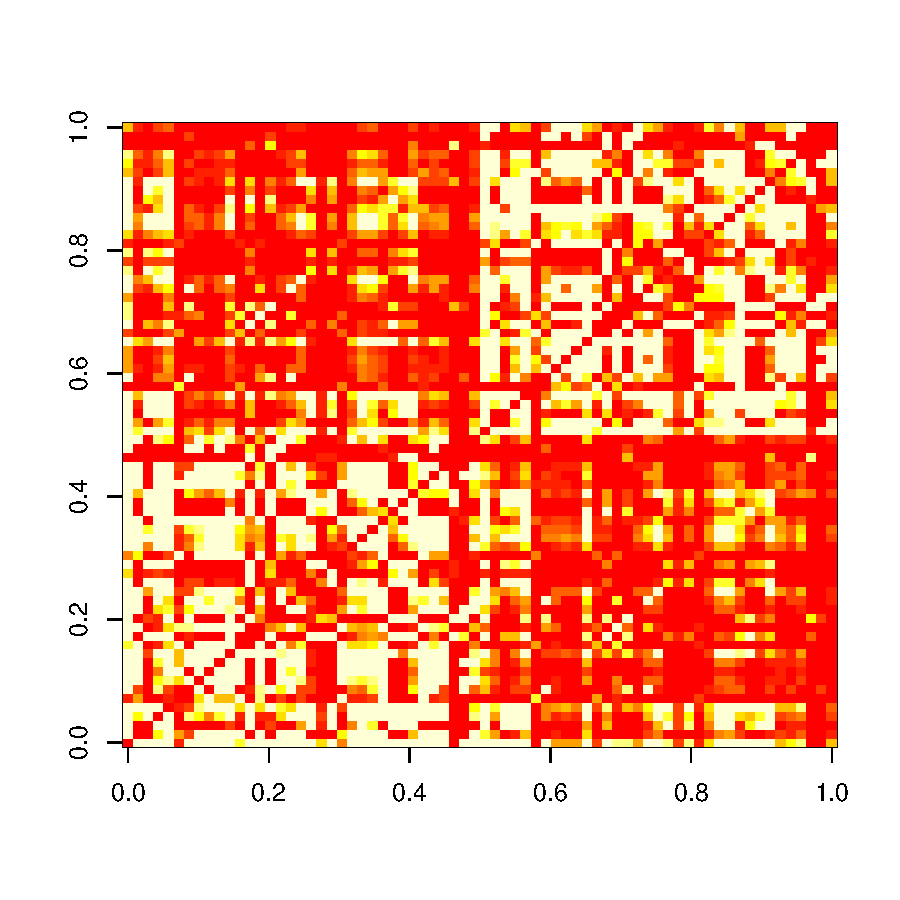
\includegraphics[width=0.455\textwidth, clip = true,  trim = 0mm 15mm 0mm 10mm]{../../figs/avgA1}
%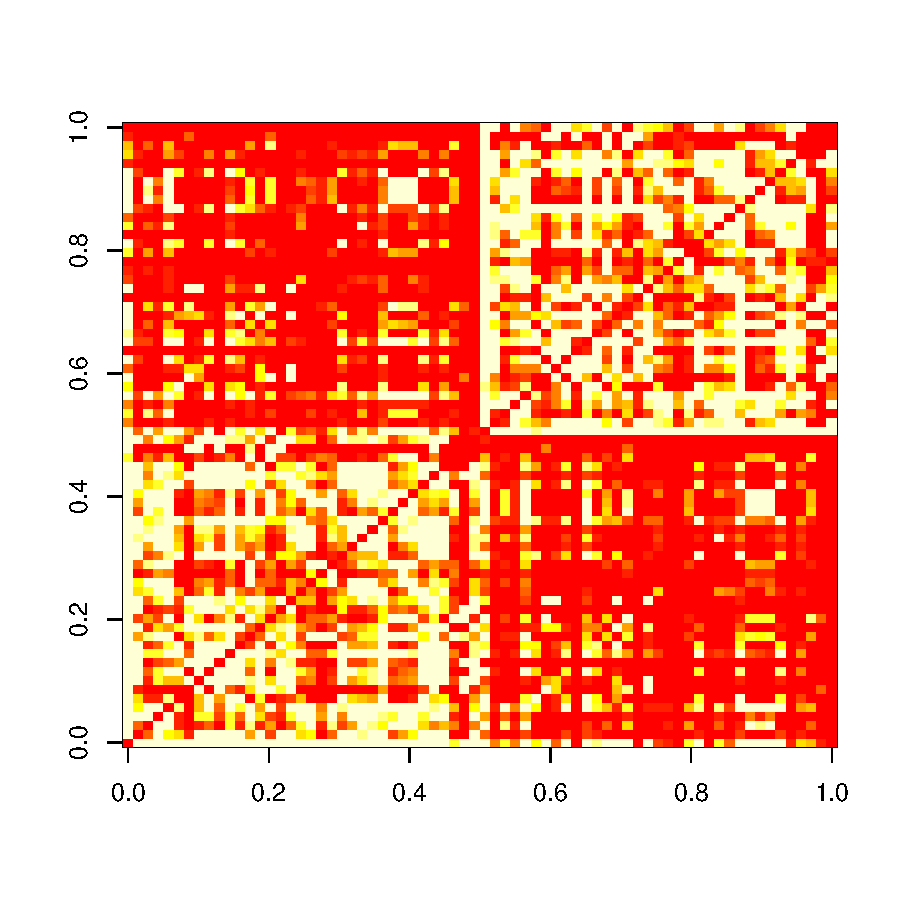
\includegraphics[width=0.4635\textwidth, clip = true, trim = 0mm 15mm 0mm 10mm ]{../../figs/avgA3}
%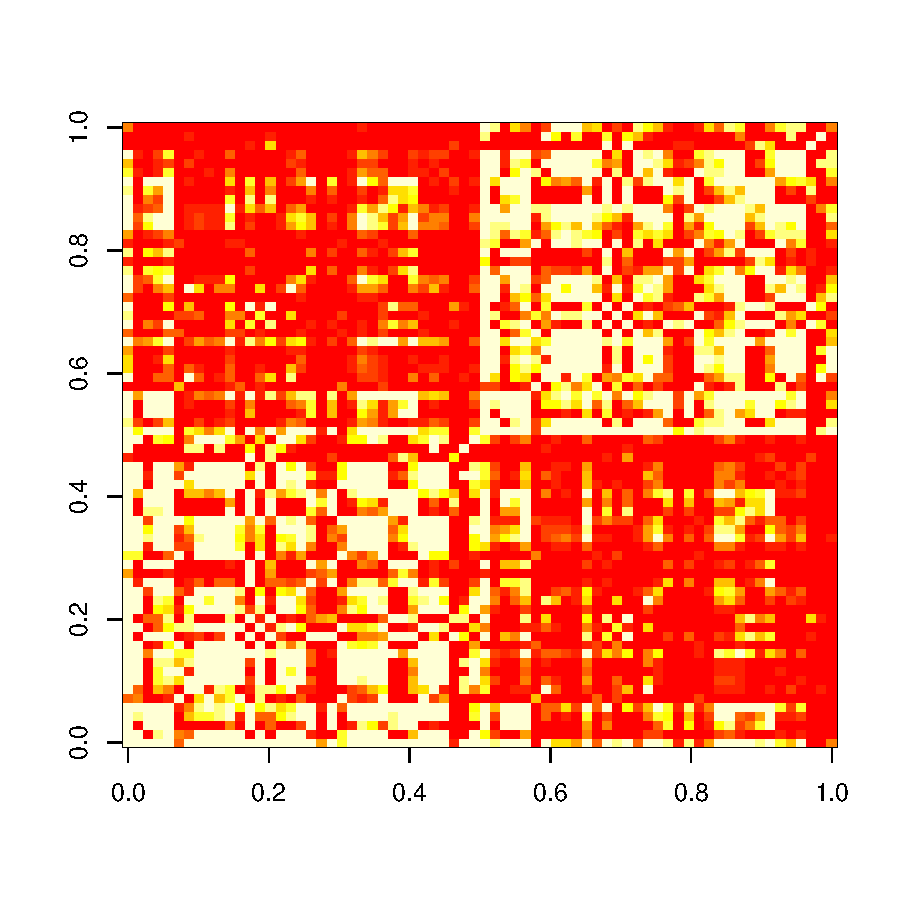
\includegraphics[width=0.455\textwidth, clip = true,  trim = 0mm 15mm 0mm 10mm]{../../figs/avgA1adjusted}
%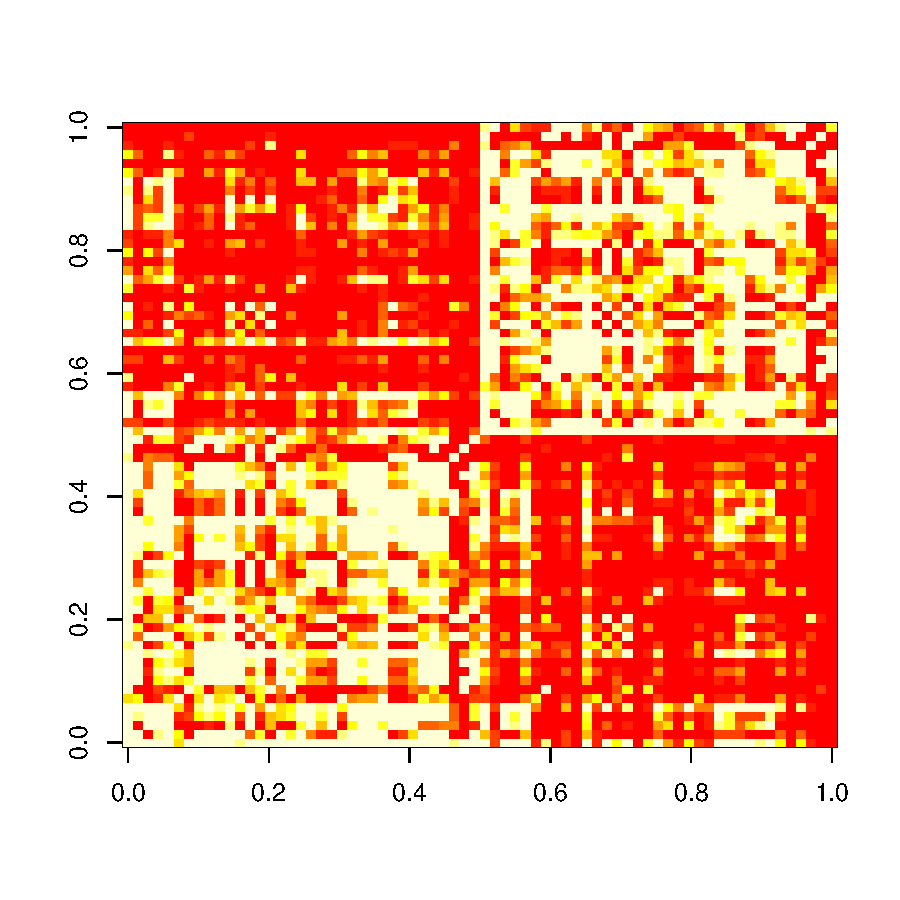
\includegraphics[width=0.4635\textwidth, clip = true, trim = 0mm 15mm 0mm 10mm]{../../figs/avgA3adjusted}
%\caption{The first row shows the average connectome of two groups, that some difference can be obsevered. The second row shows the batch effect adjusted average connectome of the two groups, that they become similar.}
%\end{cframed}
%\end{figure}
%
%
\end{document}
